\documentclass[11pt]{beamer}

% Presento style file
%\usepackage{config/presento}

% custom command and packages
% custom packages
\usepackage{textpos}
\setlength{\TPHorizModule}{1cm}
\setlength{\TPVertModule}{1cm}

\newcommand\crule[1][black]{\textcolor{#1}{\rule{2cm}{2cm}}}



\usepackage[spanish]{babel}
\selectlanguage{spanish} 
\usepackage[utf8]{inputenc}
\usepackage{default}
\usetheme{CambridgeUS}
%\usecolortheme{dolphin}
\usecolortheme{seahorse}
\usepackage{graphicx}
\usepackage{float} % supuestamente sirve para las tablas, con [H] se ponen en donde uno quiere
\restylefloat{table} % supuestamente sirve para las tablas, con [H] se ponen en donde uno quiere

\usepackage{subfig}    %para hacer figuras multiples
%\usepackage{hyperref}
\usepackage{cancel}



% Information
\title{Machine Learning en Astronom\'{\i}a}
\subtitle{Segundo seminario de Doctorado}
\author{Bruno S\'anchez \& \\
Mariano Dom\'{\i}guez}
\titlegraphic{
\includegraphics[scale=0.8]{./images/vitraux_h90.png}}
\institute{IATE - FaMAFyC} %\\
%
\includegraphics[scale=0.8]{./images/vitraux_h90.png}}
\date{\today}

\begin{document}

% Title page
\begin{frame}[plain]
\maketitle
\end{frame}

% sections in the presentation
% \begin{frame}{Resumen}
%  \begin{fullpageitemize}
%   \item \largetext{Motivaciones}
%   \item \largetext{Las diferencias de im\'agenes}
%   \item \largetext{Pipelines con Corral}
%   \item \largetext{Simulaciones de im\'agenes}
%   \item \largetext{Datos reales}
%   \item \largetext{Machine Learning}
%  \end{fullpageitemize}
% \end{frame}

\begin{frame}
\frametitle{Contenidos}
\tableofcontents%[sectionstyle=show/hide, sectionstyle=show/shaded]
\end{frame}


\section{Motivaciones}

\begin{frame}{Variabilidad el cielo}
    \begin{figure}
        \centering
        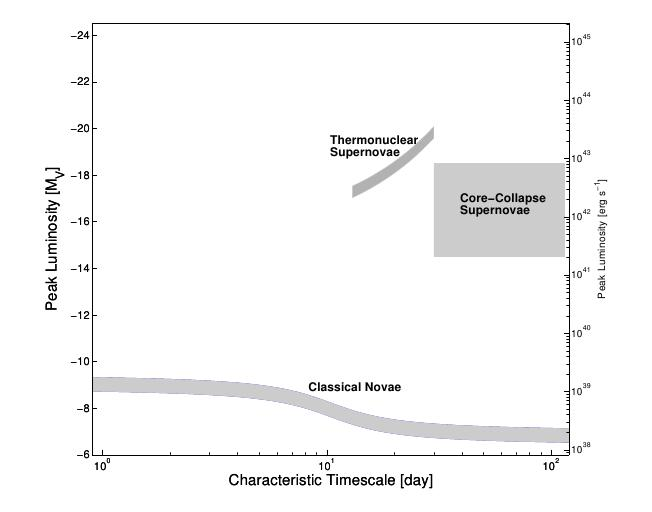
\includegraphics[width=0.7\textwidth]{./images/imgs_seminario1/diag1.jpeg}
        \caption{Diagrama de variabilidad (Kasliwal et al 2012)}
        \label{fig:diag_vacio}
    \end{figure}
\end{frame}

\begin{frame}{Variabilidad en el cielo}
    \begin{figure}
        \centering
        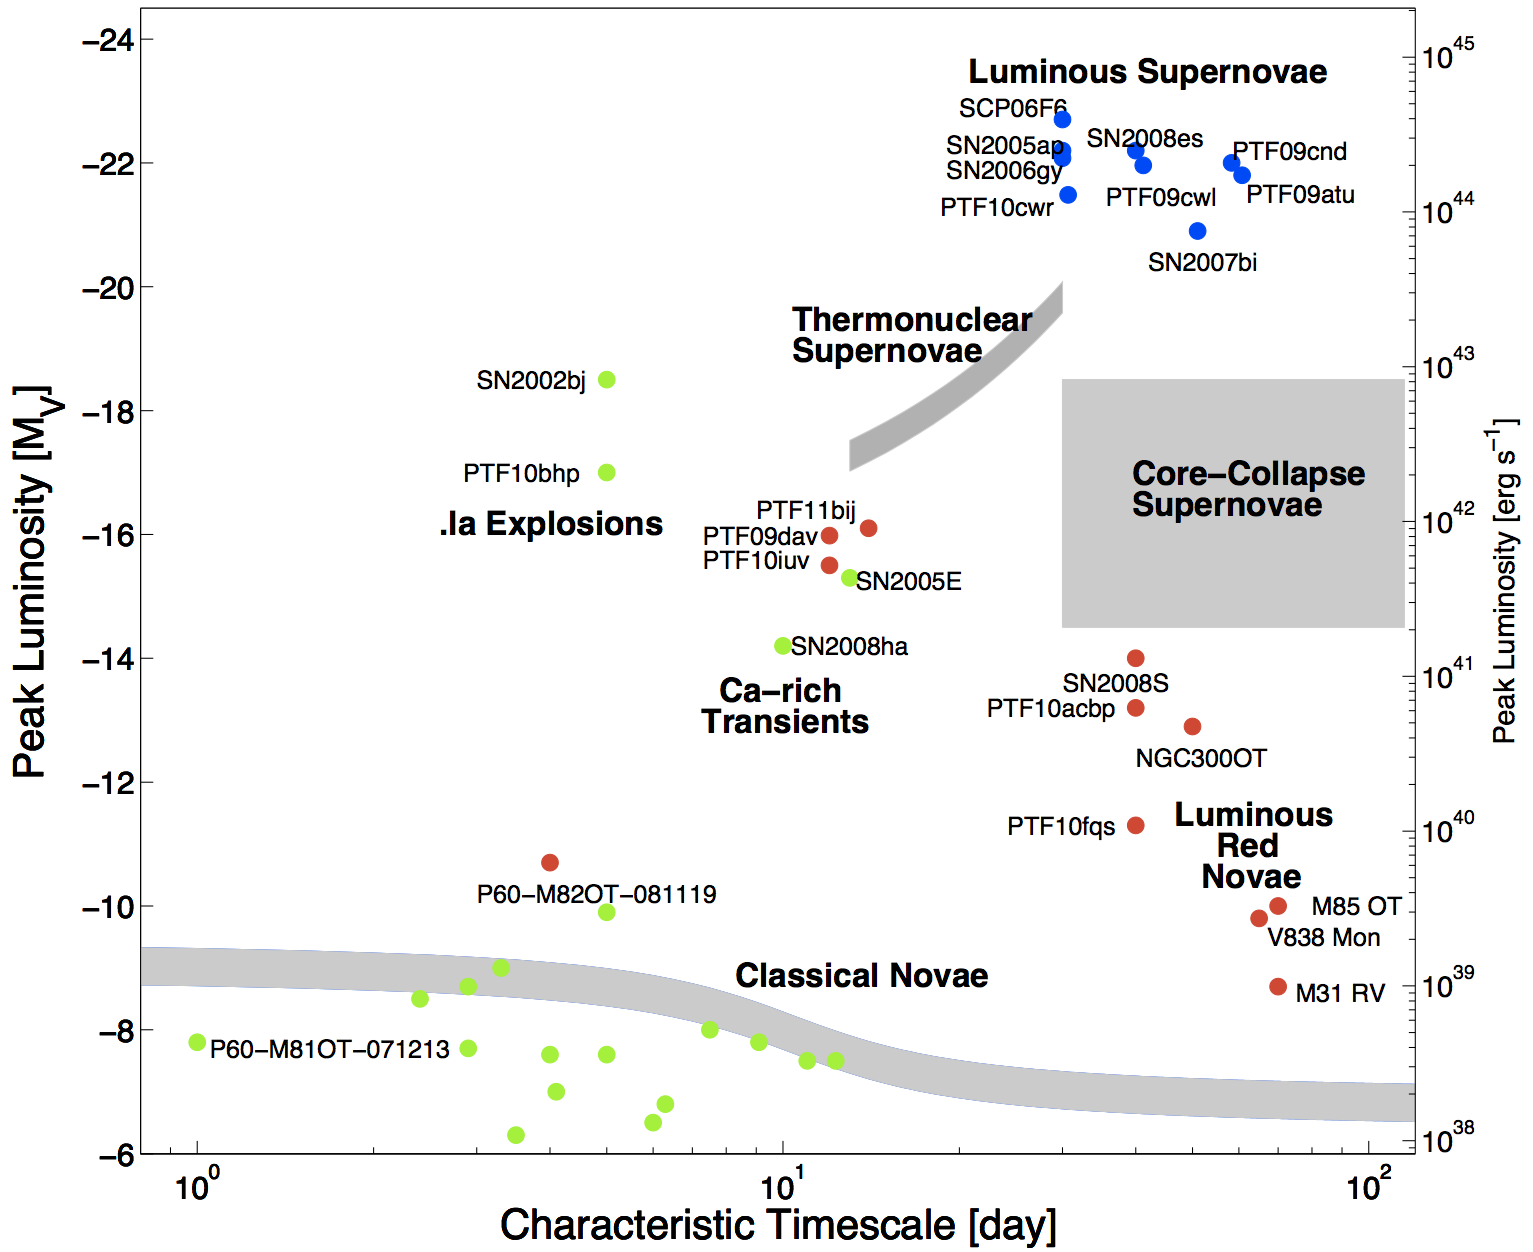
\includegraphics[width=0.65\textwidth]{./images/imgs_seminario1/taumv.png}
        \caption{Diagrama de variabilidad (Kasliwal et al 2012)}
        \label{fig:diag_lleno}
    \end{figure}
\end{frame}

\begin{frame}{Large Synoptic Survey Telescope}
    \begin{figure}
        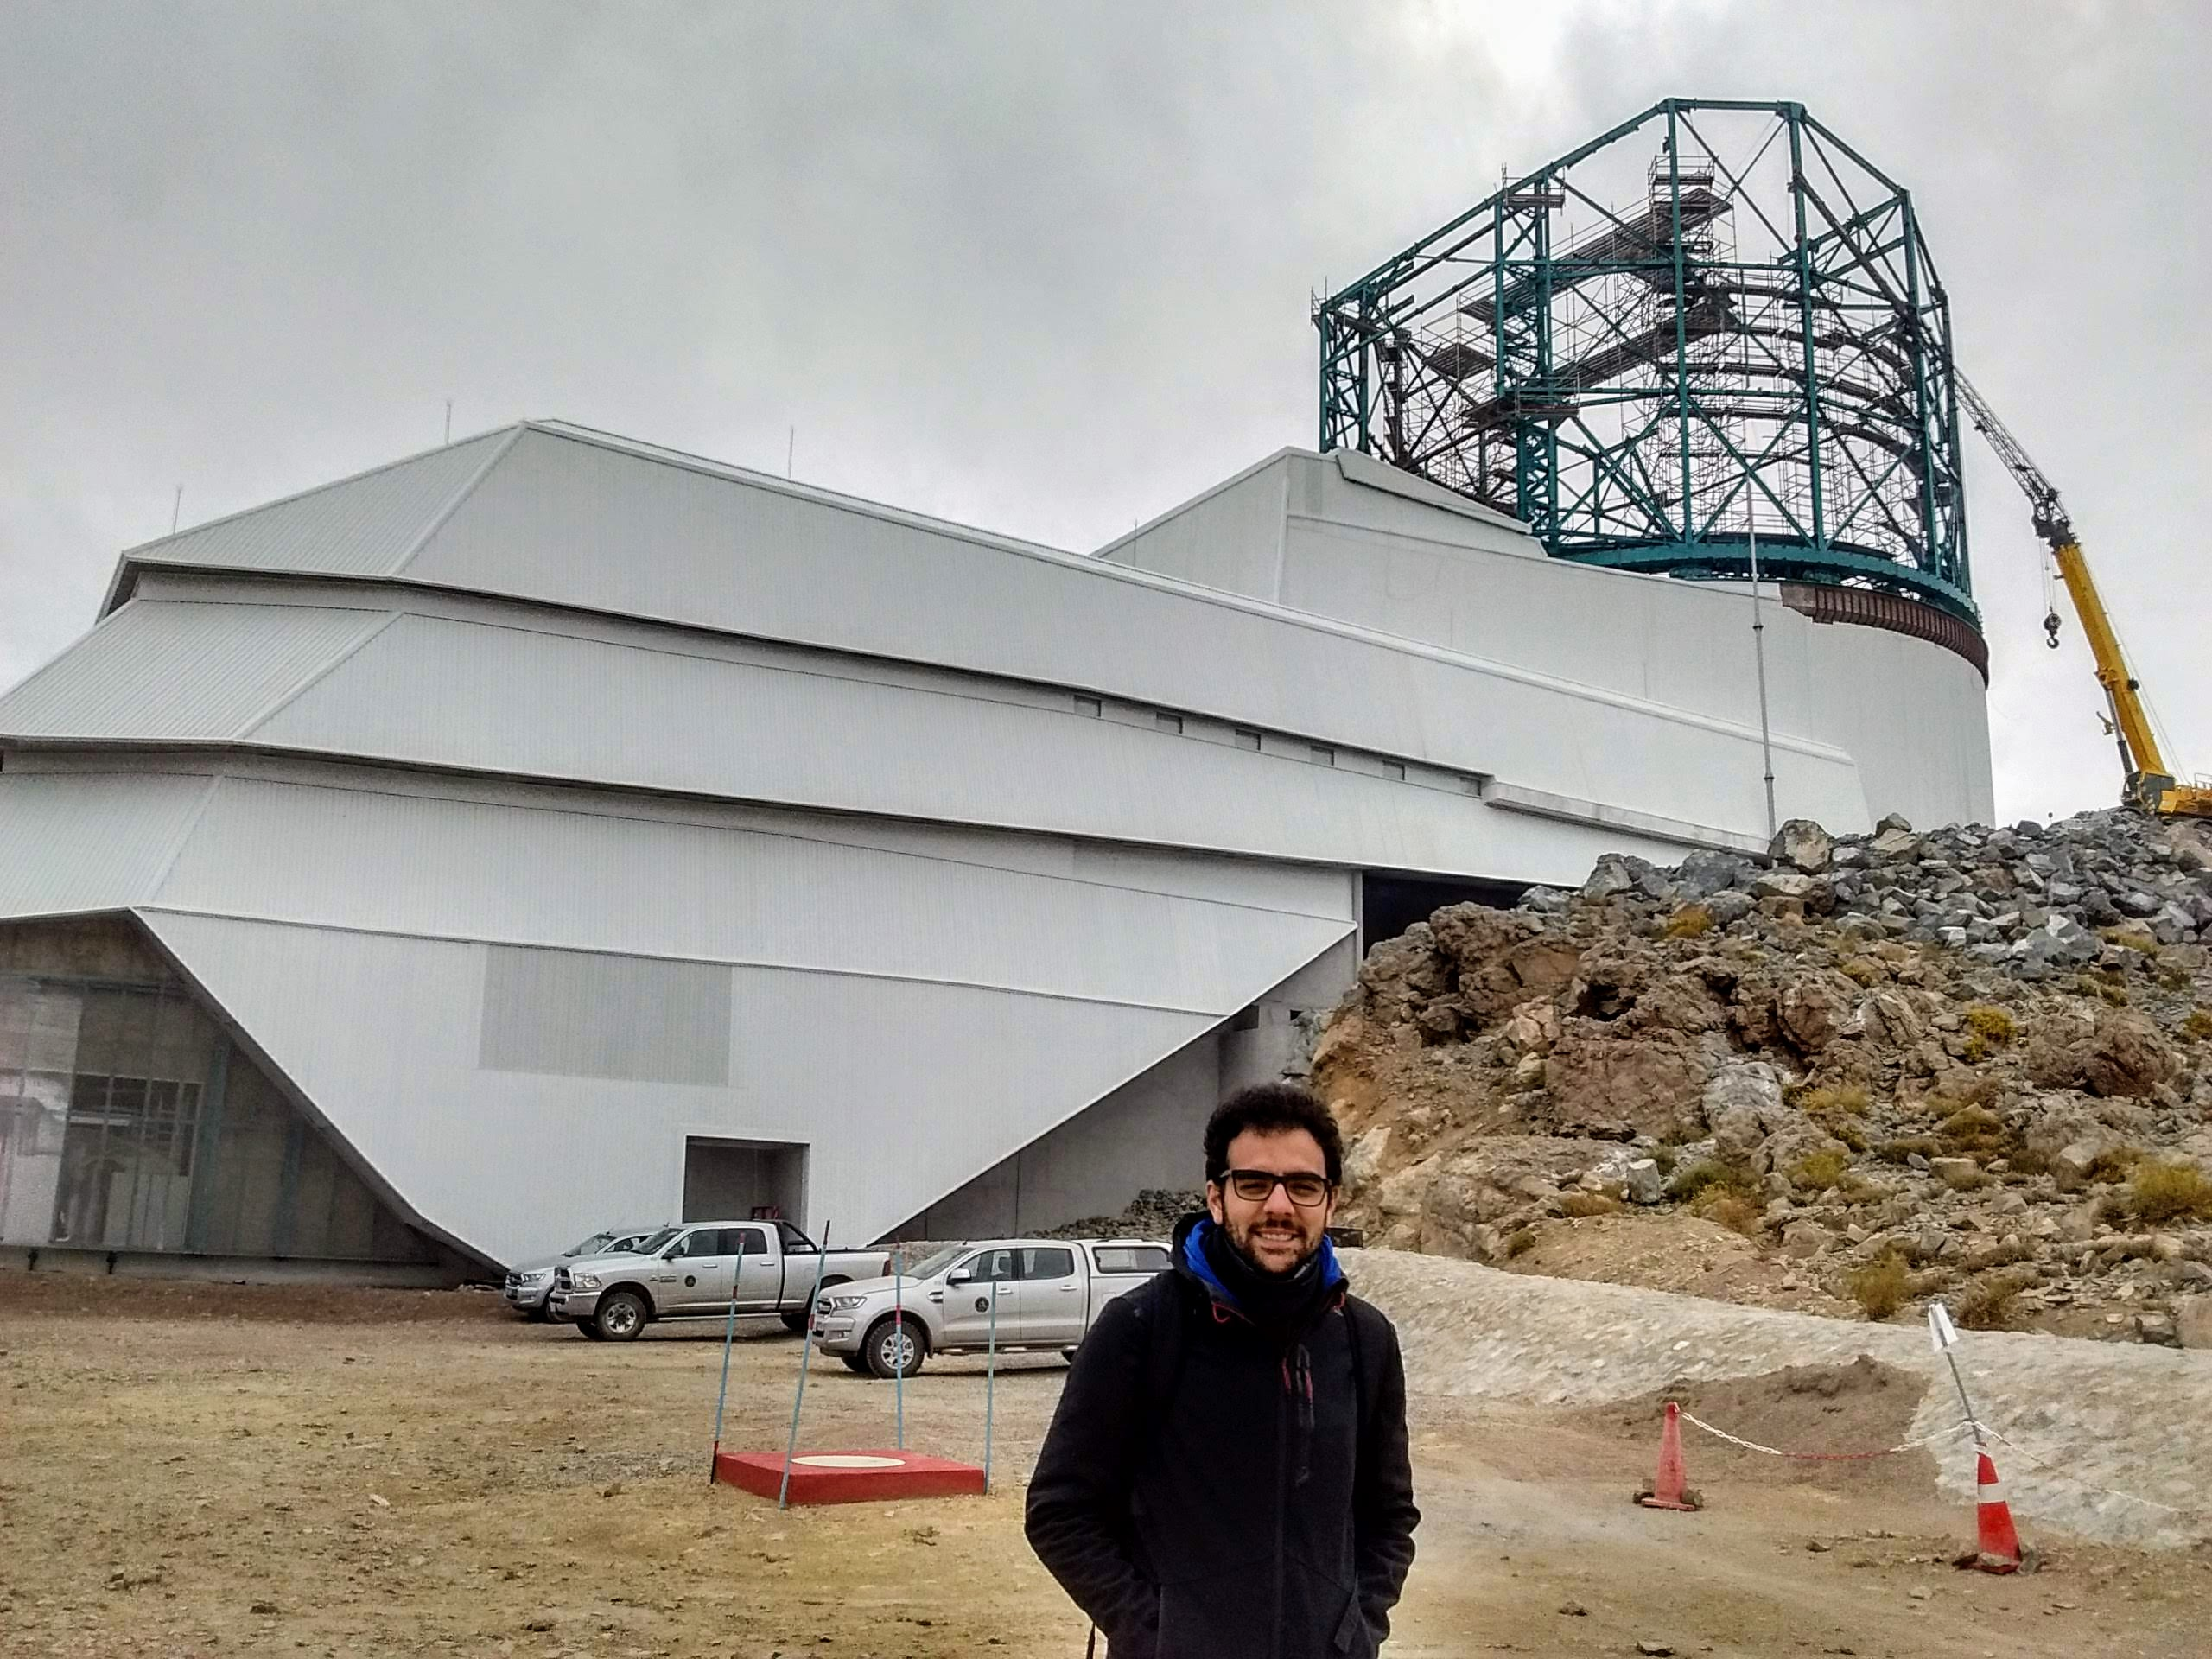
\includegraphics[width=0.45\textwidth]{./images/yo+LSST.jpg}
        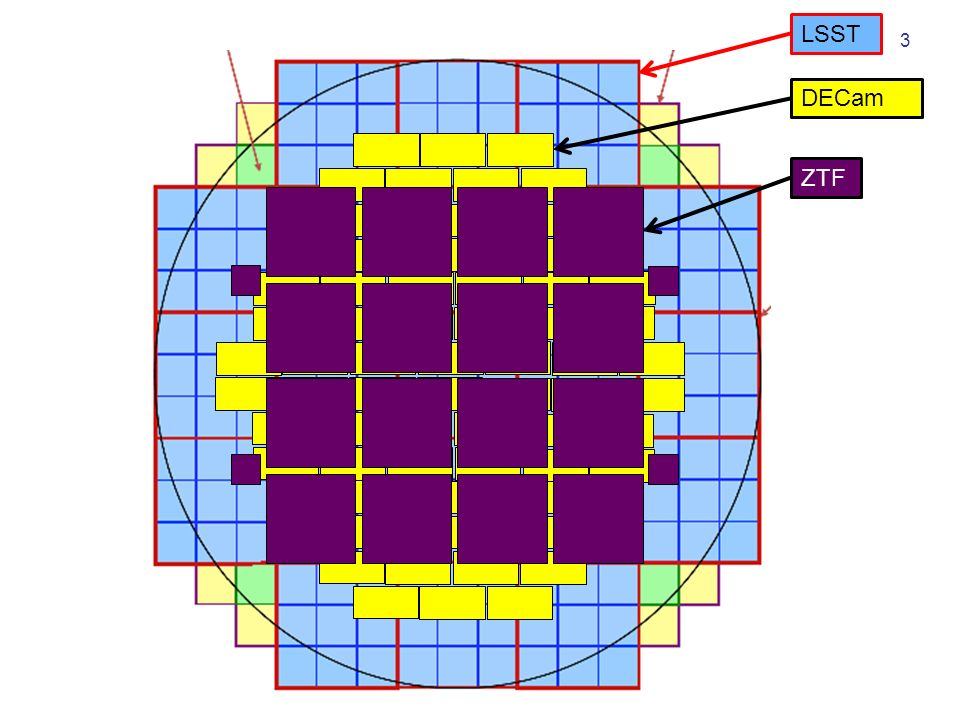
\includegraphics[width=0.45\textwidth]{./images/imgs_seminario1/LSST+DECam+ZTF.jpg}
        \caption{LSST construcci\'on y c\'amara \textit{footprint}}
        \label{fig:camaras}
    \end{figure}
\end{frame}



\begin{frame}{Las diferencias de im\'agenes (DIA)}
Pros \& Cons
   \begin{exampleblock}{Localizado}
   Se pueden encontrar eventos dentro de objetos extendidos
   \end{exampleblock}
   \pause
   \begin{exampleblock}{Sensible}
   Se pueden detectar objetos d\'ebiles
   \end{exampleblock}
   \pause
   \begin{alertblock}{Artefactos de la sustracci\'on}
   La operaci\'on tiene resultados inestables
   \end{alertblock}
   
\end{frame}

\begin{frame}{Distintos tipos de operaciones DIA}
    Primeros intentos: \cite{phillips_registering_1995}
    
    Hoy existen diferentes t\'ecnicas de sustracci\'on de im\'agenes:
    \begin{itemize}
        \item Alard \& Lupton \cite{alard_method_1998}
        \item Bramich \cite{bramich_new_2008}
        \item Zackay, Ofek and Gal-Yam \cite{zackay_proper_2016}
    \end{itemize}
\end{frame}

\begin{frame}{Conex\'on con el ML}
    A pesar de ser diferentes las t\'ecnicas, 
    todas poseen defectos:
    \begin{figure}
        \centering
        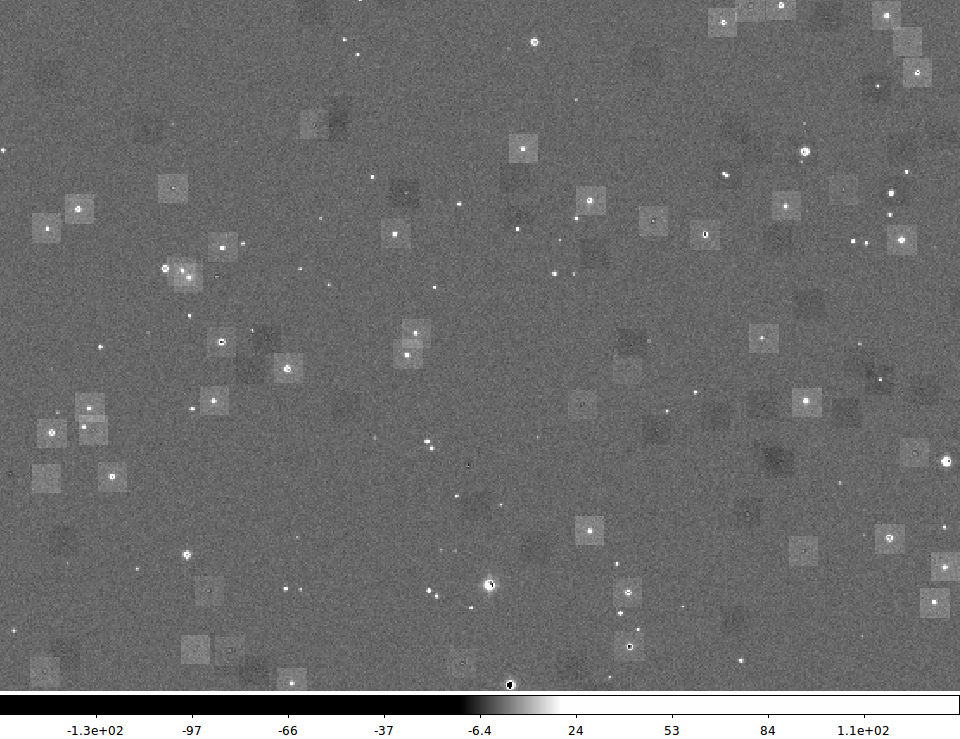
\includegraphics[width=0.33\textwidth]{images/diff.png}
        %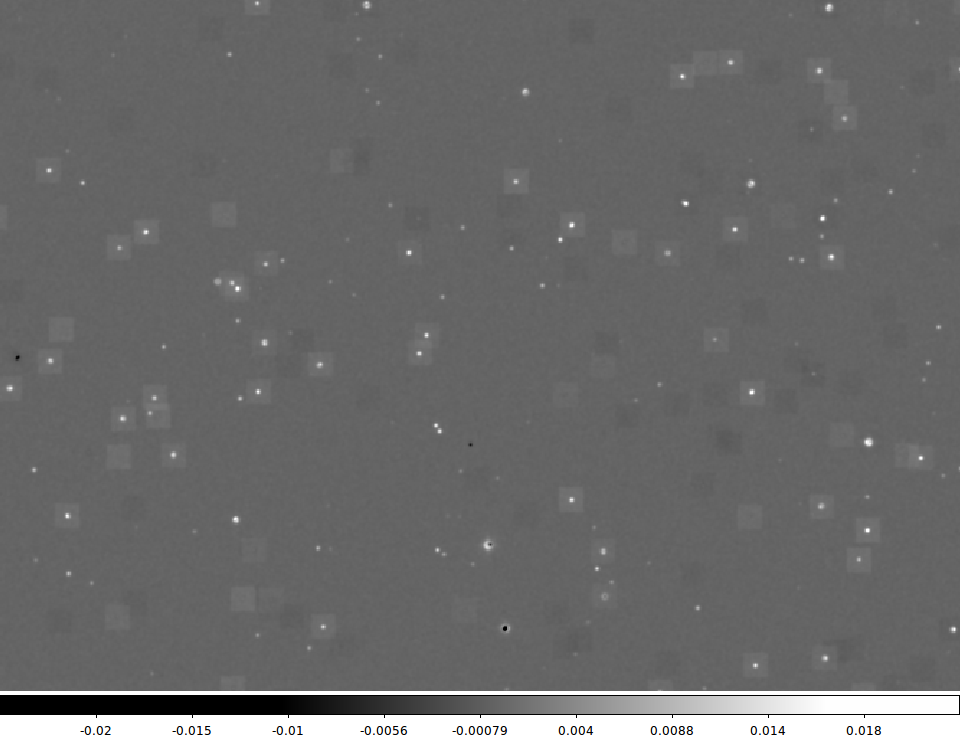
\includegraphics[width=0.23\textwidth]{images/s_diff.png}
        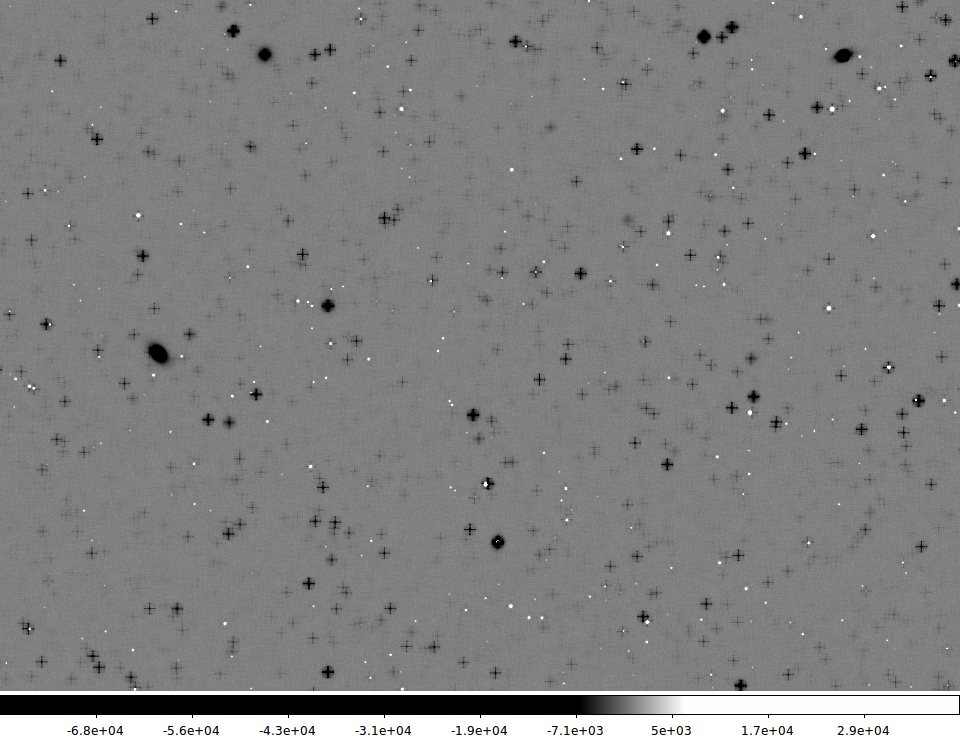
\includegraphics[width=0.33\textwidth]{images/diff_ois.png}
        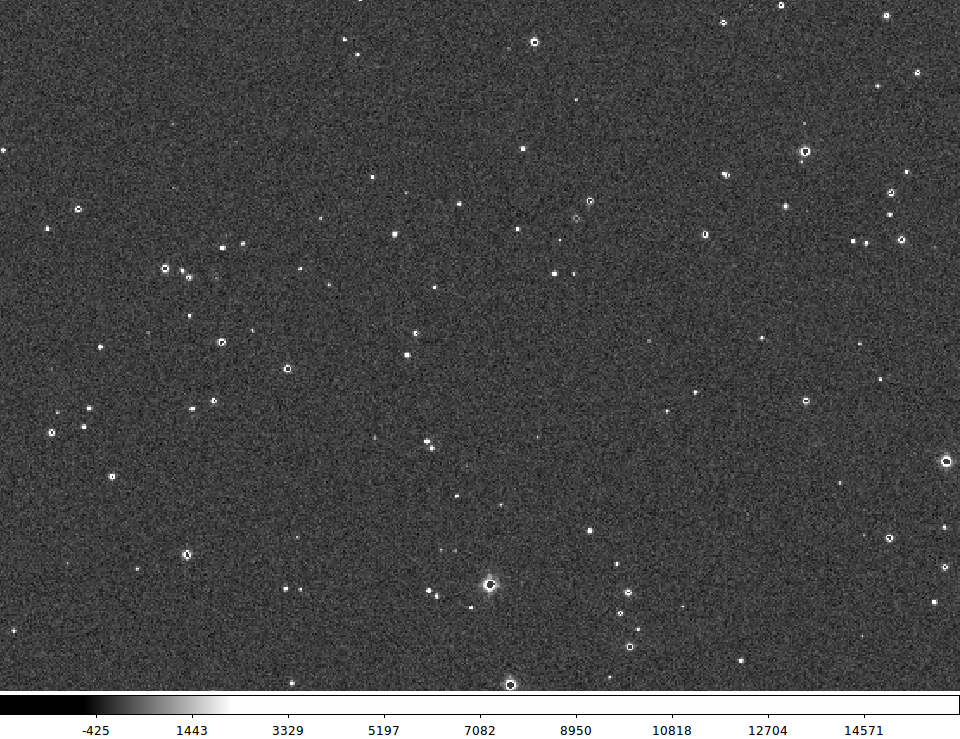
\includegraphics[width=0.33\textwidth]{images/diff_hot.png}
        \caption{Izq. Zackay, centro Bramich, der. A\&Lupton.}
        \label{fig:restas}
    \end{figure}
    \end{frame}




\section{Machine Learning}

\begin{frame}{Algunas definiciones del ML}
    A. Samuel (1956):
    \begin{quote}
        Un campo de estudio que le da la habilidad a una computadora de aprender sin ser explicitamente programada
    \end{quote}
    T. Mitchel (1998):
    \begin{quote}
        Estudio de algoritmos que mejoran la perfomance $P$ en alguna tarea $T$ con la experiencia $E$
    \end{quote}
\end{frame}

\begin{frame}{Un breve esquema}
    %Como forma de trabajo se cambia totalmente la mec\'anica:
    \begin{figure}
        \centering
        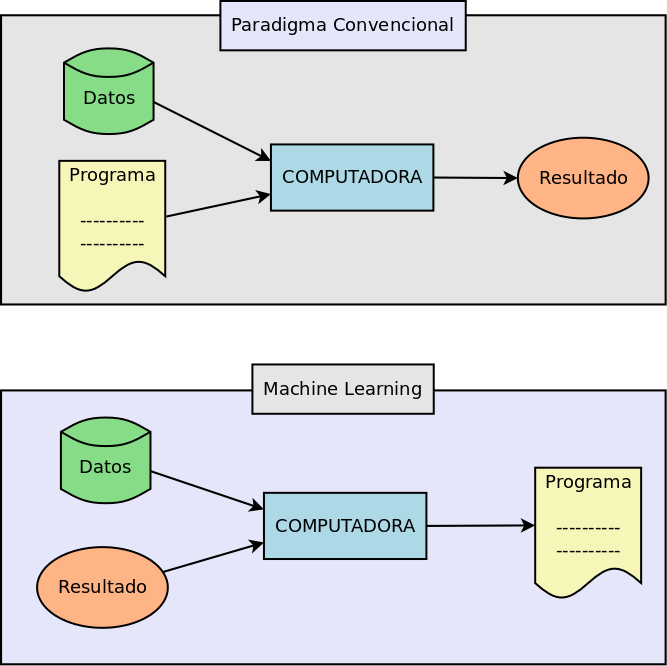
\includegraphics[width=0.6\textwidth]{images/ML_vs_programming.png}
        %\caption{}
        \label{fig:ML_vs_conventional}
    \end{figure}
\end{frame}

\begin{frame}{Tipos de ML}
    \begin{itemize}
        \item Aprendizaje supervisado 
        \item Aprendizaje \textbf{NO}-supervisado
        \item Aprendizaje semi-supervisado
    \end{itemize}
\end{frame}

\begin{frame}{Algoritmos de Machine Learning}
    Un algoritmo se compone de tres elementos:
    \begin{itemize}%[<+->]
        \item Representaci\'on\only<2>{: \textit{el tipo de modelo que utilizaremos para predecir}}
        \item Evaluaci\'on\only<3>{: \textit{la funci\'on que maximizaremos para que nuestro modelo pueda aprender}}
        \item Optimizaci\'on\only<4>{: \textit{la estrategia de b\'usqueda de los par\'ametros que maximizan la funci\'on de evaluaci\'on}}
    \end{itemize}

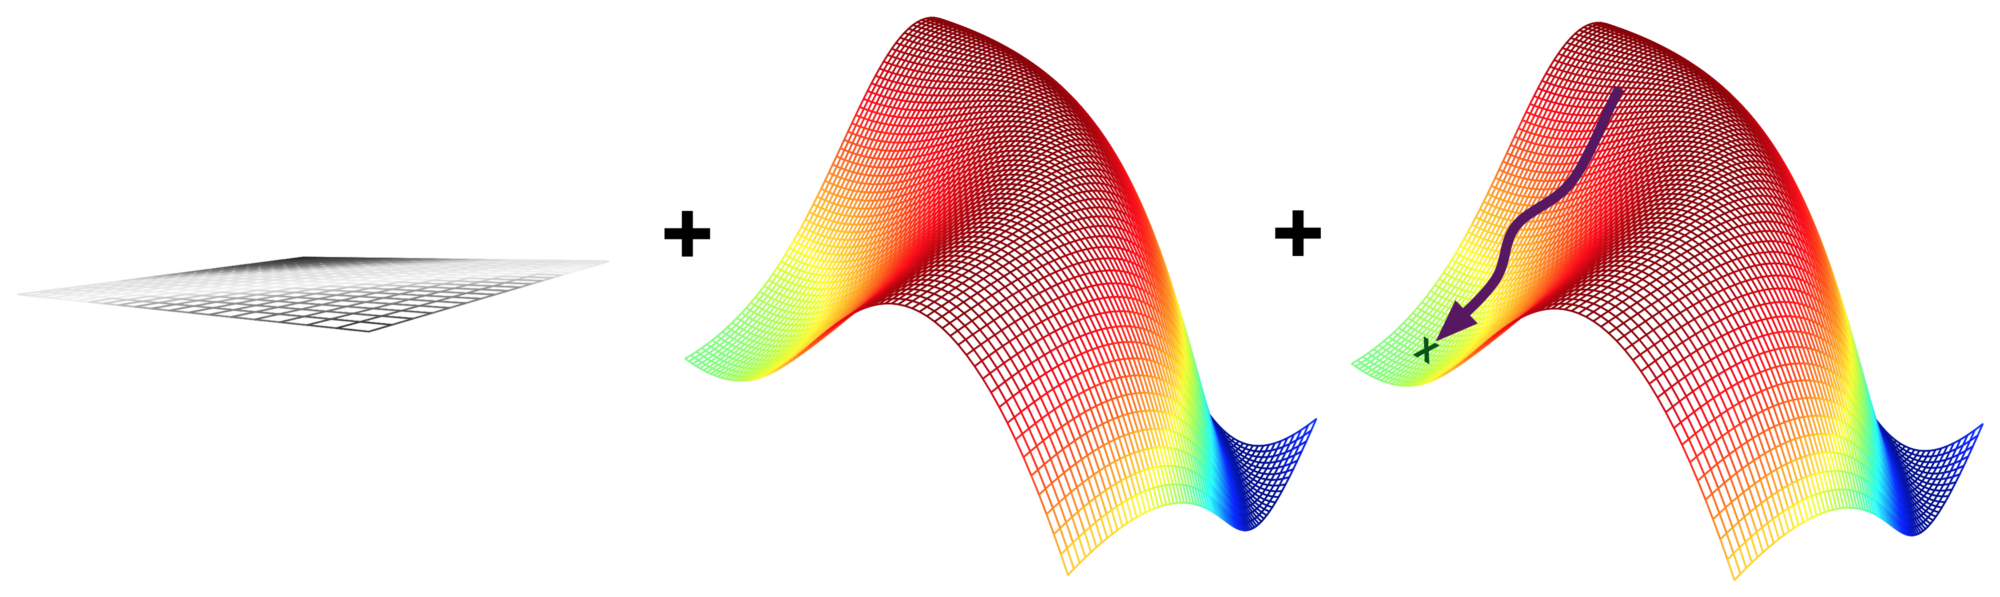
\includegraphics[width=0.9\textwidth]{images/representation+evaluation+optimization.png}

\end{frame}

\begin{frame}{Ejemplos de representacion}
\begin{itemize}[<+->]
    \item Regresi\'on lineal: simplemente el ajuste de una recta a nuestros datos $$y_i = a x_i + b$$
    \item Naive Bayes: utiliza el teorema de bayes para estimar probabilidades
    $$P(c=c_i|\vec{f}) = \frac{P(\vec{f}|c=c_i)P(c=c_i)}{P(\vec{f})}$$
    \item \'Arboles de decisi\'on: una estructura de dendograma
    \begin{center}
    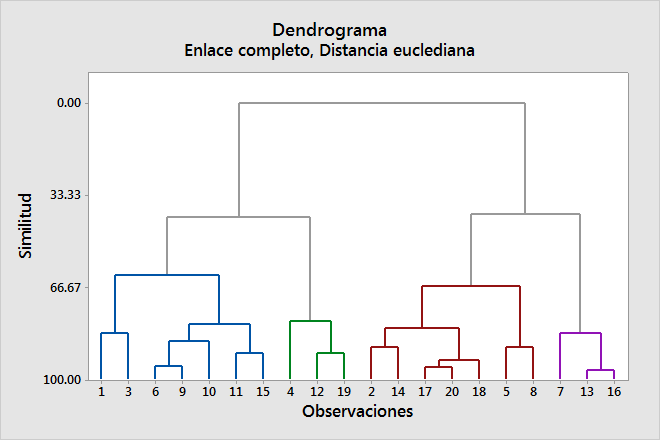
\includegraphics[width=0.45\textwidth]{images/cluster_obs_dendrogram_with_final_partition_glove_testers.png}    
    \end{center}
\end{itemize}    
\end{frame}



\begin{frame}{Evaluaci\'on: Tipos de errores}
Los errores en ML se extraen de la llamada \textbf{Matriz de Confusi\'on}
\small
\begin{center}
\begin{tabular}{|c|c|l|}
\hline
- & \multicolumn{2}{c|}{Decisi\'on}\\
\hline \hline
Condici\'on Real & Rechazar $H_0$ & \multicolumn{1}{c|}{Mantener $H_0$}\\
\hline
$H_0$ Verdadera & Error de Tipo I & \multicolumn{1}{c|}{Acierto}\\
\hline
$H_0$ Falsa & Acierto & \multicolumn{1}{c|}{Error de Tipo II}\\
\hline
\end{tabular}
\end{center}
\end{frame}

\begin{frame} \frametitle{M\'etricas}
 %Los estad\'{i}sticos que miden el rendimiento de un test de decisi\'on son FDR, TPR, y FPR.
 \small
\begin{itemize}
 \item \textbf{FDR} (o \textit{Tasa de Falsos Descubrimientos}) corresponde a la probabilidad 
 de cometer un error de Tipo I habiendo obtenido como resultado el rechazo de $H_0$
 \item \textbf{TPR} (o \textit{Tasa de Positivos Verdaderos}) corresponde a la probabilidad de 
 rechazar la $H_0$ dado que es falsa, o bien uno menos la probabilidad de cometer un Error de Tipo I
\item \textbf{FPR} (o \textit{Tasa de Falsos Positivos}) el cual es la probabilidad de cometer un error de Tipo II
\end{itemize}
\end{frame}


\begin{frame} \frametitle{Figura de M\'erito}
 \small
 \begin{columns}[T]
\begin{column}{0.48\textwidth}
 Las tasas de FPR y TPR dependen del valor umbral que se aplique a un dado m\'etodo.\\ 
 Las tasas de FPR y TPR poseen un balance que se caracteriza por la \textit{Respuesta Caracter\'{i}stica del Operador}.\\ 
 AUC (\textit{\'Area Bajo la Curva})
 \end{column}
 \begin{column}{0.55\textwidth}
 \begin{figure}
 \centering
 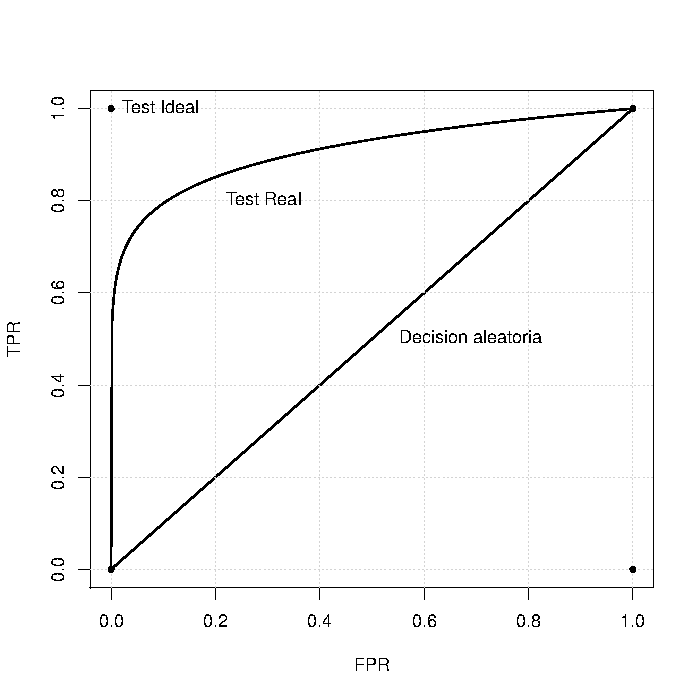
\includegraphics[width=\textwidth]{./images/imgs_seminario1/ROC.png}
 % ROC.ps: 504x504 pixel, 72dpi, 17.78x17.78 cm, bb=0 0 504 504
 \caption{\scriptsize{Curva ROC}}
 %\label{fig:roc}
\end{figure}\pause
\end{column}
 \end{columns}
\end{frame}



% \begin{frame}{Open Source Fonts}
%  \begin{fullpageitemize}
%   \item {\montserratfont This is Montserrat}
%   \item {\notosansfont This is Noto Sans}
%   \item {\latolightfont This is Lato (light)}
%   \item {\inconsolatafont This is inconsolata}
%   \item \textsc{This is Alegreya Sans small caps}
%  \end{fullpageitemize}
% \end{frame}

% \begin{frame}{Color Palette}
%  \begin{center}
%   \crule[colordgray] \crule[colorhgray] \crule[colorblue] \crule[colorgreen] \crule[colororange]
%  \end{center}
% \end{frame}

% \framecard[colorgreen]{{\color{white}\hugetext{BIG BOLD TEXT}}}

% \framepic[0.8]{images/skeleton}{
%  \begin{textblock}{7}(7,2.5)
%     {\color{colorblue}\hugetext{\textbf{RUN!}}}
%  \end{textblock}
% }


\begin{frame}[allowframebreaks]
        \frametitle{Referencias}
        \tiny
        \bibliographystyle{apalike}
        \bibliography{bibliography.bib}
\end{frame}
\end{document}